% Fine branch pipeline detailed figure
% Compile: pdflatex fine_pipeline.tex
% Inline:  % Fine branch pipeline detailed figure
% Compile: pdflatex fine_pipeline.tex
% Inline:  % Fine branch pipeline detailed figure
% Compile: pdflatex fine_pipeline.tex
% Inline:  % Fine branch pipeline detailed figure
% Compile: pdflatex fine_pipeline.tex
% Inline:  \input{figures/fine_pipeline.tex}
%
% 配套 ctx_pipeline.tex / coarse_pipeline.tex，把 fine iGPT 分支 forward 全路径
% 在「张量 shape + dtype + 三路 additive 注入 + GPT block 内部」三个层面具象化。
\documentclass[tikz,border=10pt]{standalone}
\usepackage{tikz}
\usepackage{amsmath,amssymb}
\usepackage{xcolor}
\usetikzlibrary{positioning,arrows.meta,calc,fit,backgrounds,shapes.geometric,
                decorations.pathreplacing,patterns}

\begin{document}
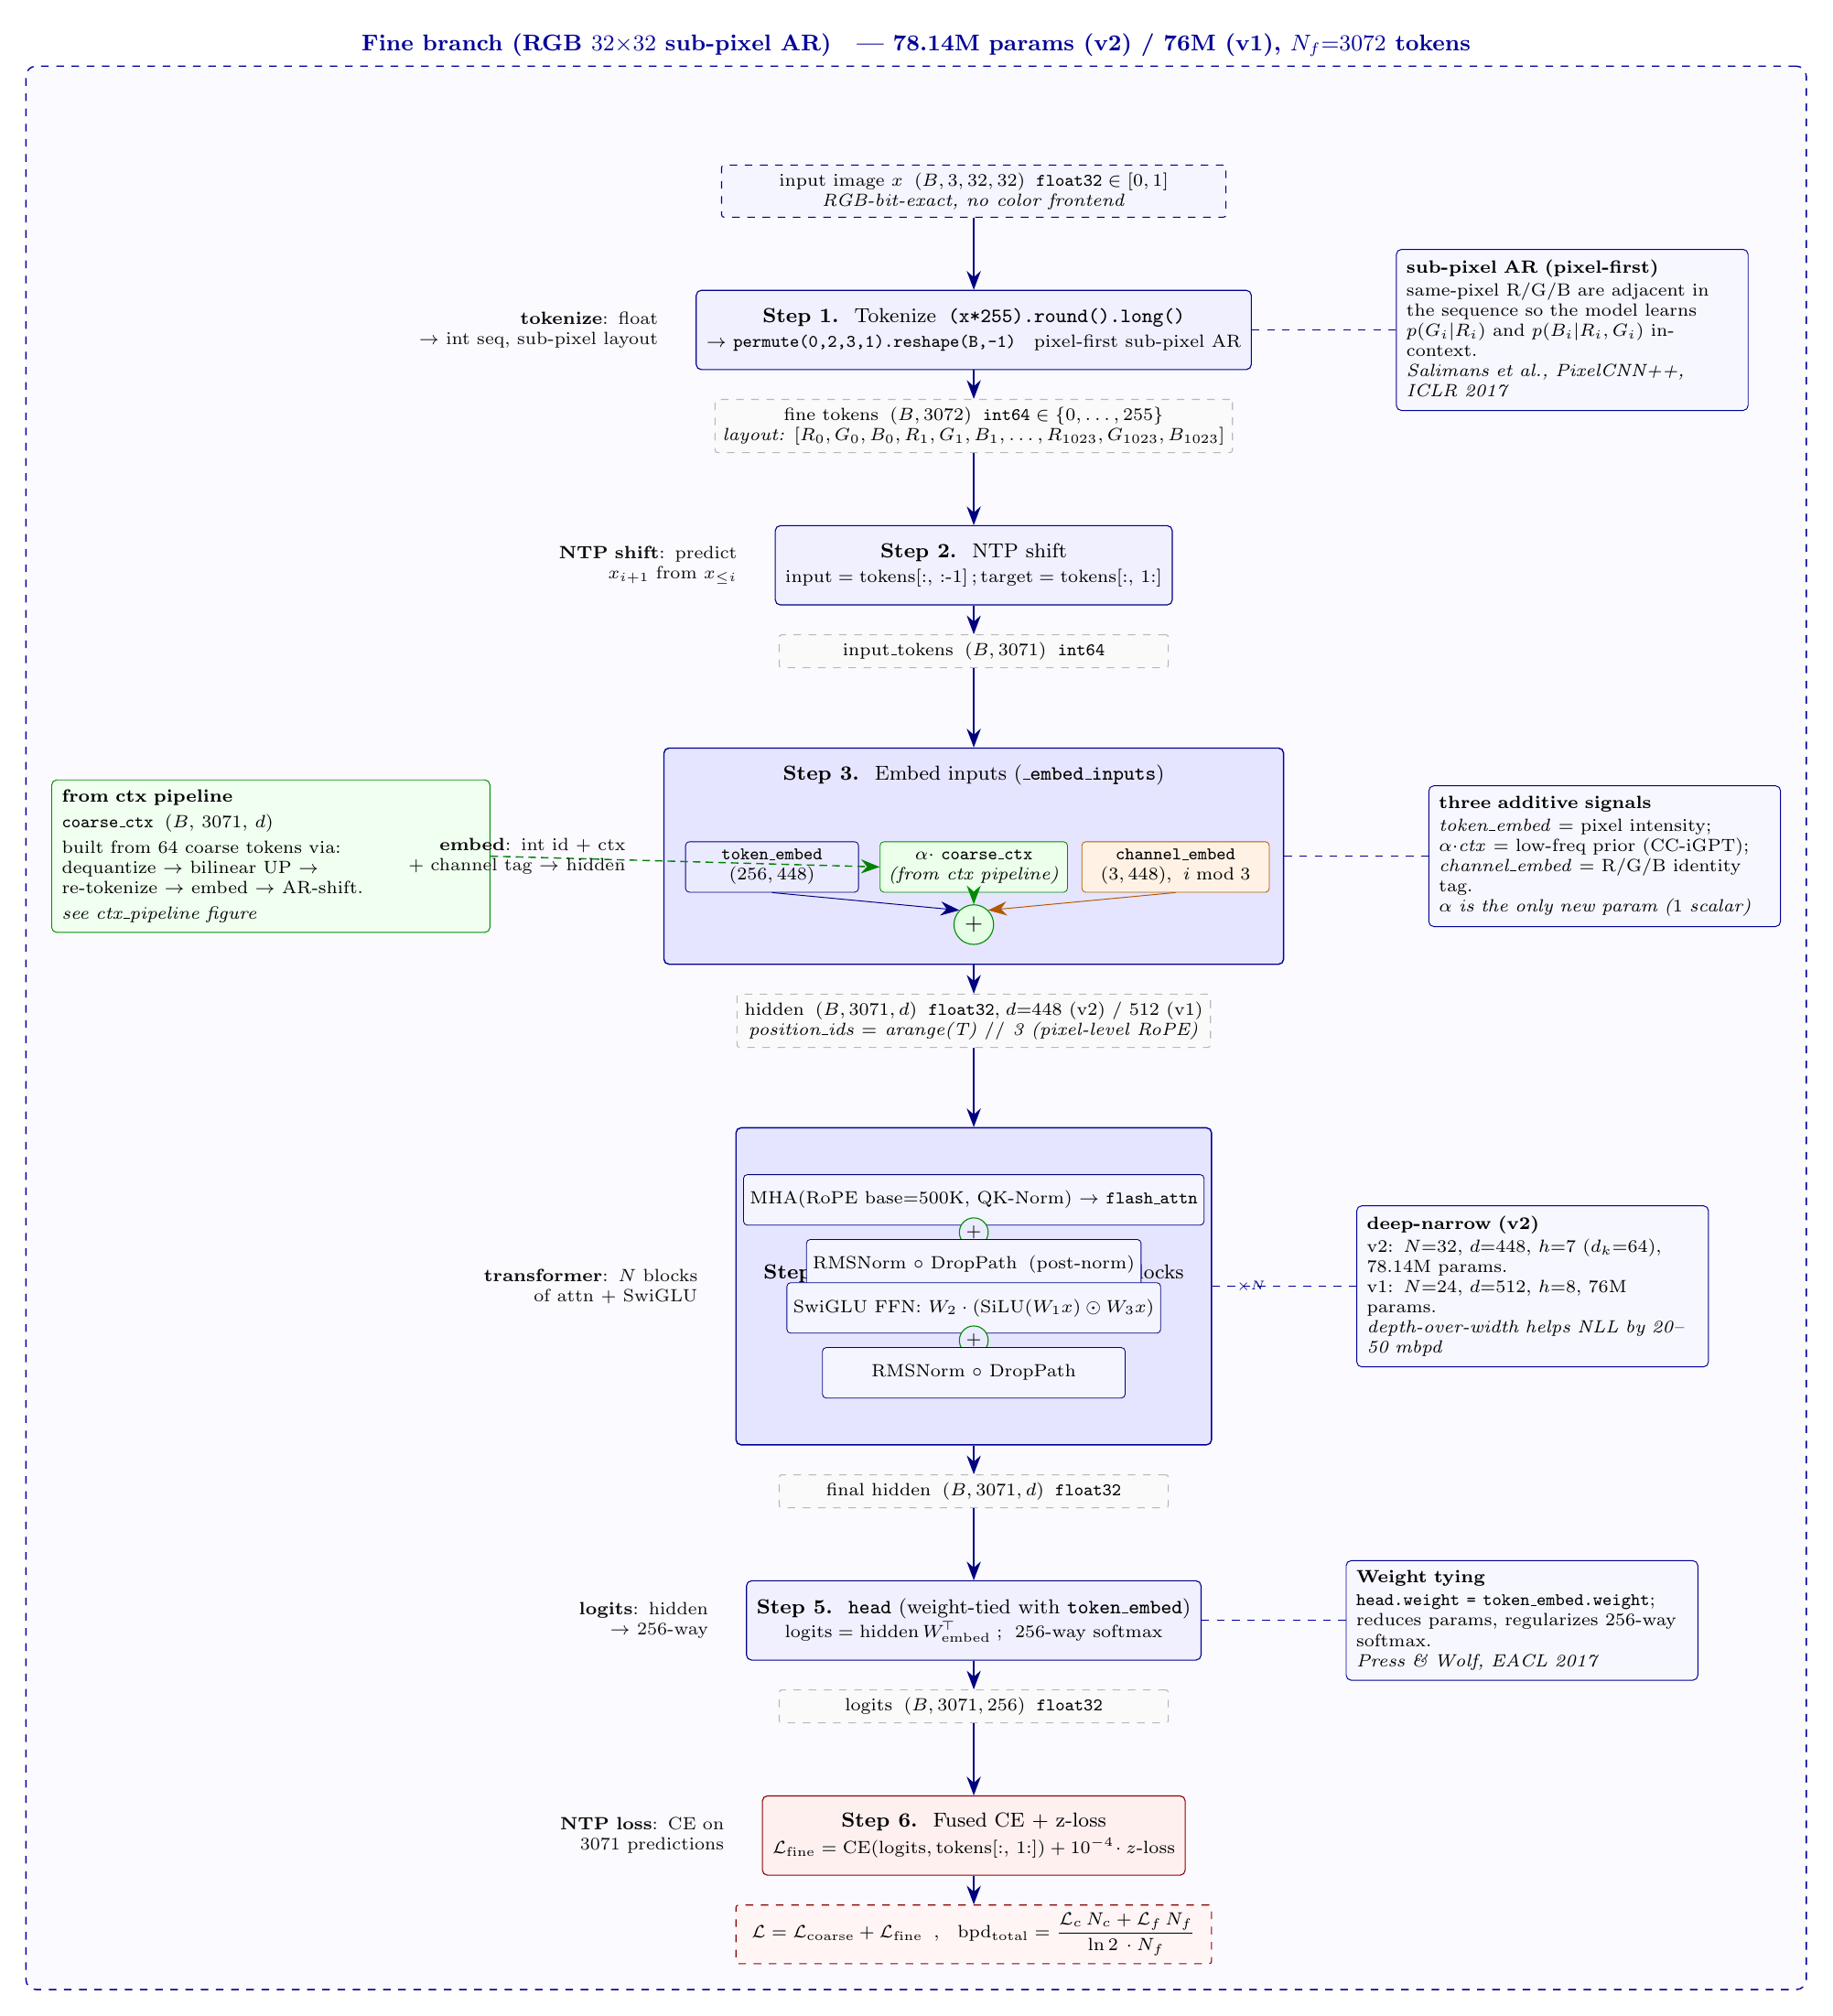
\begin{tikzpicture}[
    font=\footnotesize,
    >={Stealth[length=2.6mm]},
    node distance=10mm and 14mm,
    stepbox/.style ={draw, rounded corners=2pt, align=center,
                     minimum height=11mm, minimum width=54mm,
                     inner sep=4pt, fill=blue!6, draw=blue!55!black,
                     line width=0.4pt},
    blockbox/.style={draw, rounded corners=2pt, align=center,
                     minimum height=14mm, minimum width=54mm,
                     inner sep=4pt, fill=blue!10, draw=blue!60!black,
                     line width=0.5pt},
    sublayer/.style={draw, rounded corners=1.5pt, align=center,
                     minimum height=7mm, minimum width=36mm,
                     inner sep=2.5pt, fill=blue!4, draw=blue!50!black,
                     font=\scriptsize, line width=0.3pt},
    tensor/.style  ={draw, dashed, rounded corners=1pt, align=center,
                     fill=gray!4, draw=gray!55, font=\scriptsize,
                     inner sep=3pt, minimum width=54mm},
    lossbox/.style ={draw, rounded corners=2pt, align=center,
                     minimum height=11mm, minimum width=54mm,
                     inner sep=4pt, fill=red!6, draw=red!55!black,
                     line width=0.4pt},
    callout/.style ={draw=blue!60!black, rounded corners=2pt,
                     fill=blue!3, align=left, font=\scriptsize,
                     inner sep=4pt, line width=0.35pt},
    inject/.style  ={draw, circle, inner sep=0.5pt, fill=green!10,
                     draw=green!55!black, minimum size=5.5mm, font=\small},
    flow/.style    ={->, line width=0.55pt, blue!50!black},
    sidearrow/.style={->, line width=0.5pt, green!50!black, densely dashed},
]

% =========================================================
% TOP: invisible top spacer to host the fnbox label safely
% =========================================================
\node[minimum width=70mm, minimum height=8mm, inner sep=0pt]
     (topspacer) {};

% =========================================================
% TOP: input image
% =========================================================
\node[tensor, fill=blue!4, draw=blue!55!black, minimum width=70mm,
      below=2mm of topspacer]
     (xin) {input image $x$\;\;$(B,3,32,32)$\;\;\texttt{float32}\;$\in[0,1]$\\
            \textit{RGB-bit-exact, no color frontend}};

% =========================================================
% Step 1 -- tokenize (sub-pixel AR, pixel-first)
% =========================================================
\node[stepbox, below=10mm of xin] (s1)
     {\textbf{Step 1.} \;Tokenize\;\;\texttt{(x*255).round().long()}\\
      \scriptsize $\to$ \texttt{permute(0,2,3,1).reshape(B,-1)}\;\;
      pixel-first sub-pixel AR};
\node[tensor, below=4mm of s1] (t1)
     {fine tokens\;\;$(B,3072)$\;\;\texttt{int64}\;$\in\{0,\dots,255\}$\\
      \textit{layout: $[R_0,G_0,B_0,R_1,G_1,B_1,\dots,R_{1023},G_{1023},B_{1023}]$}};

% =========================================================
% Step 2 -- NTP shift
% =========================================================
\node[stepbox, below=10mm of t1] (s2)
     {\textbf{Step 2.} \;NTP shift\\
      \scriptsize input\;$=$\;tokens[:, :-1]\,;\,target\;$=$\;tokens[:, 1:]};
\node[tensor, below=4mm of s2] (t2)
     {input\_tokens\;\;$(B,3071)$\;\;\texttt{int64}};

% =========================================================
% Step 3 -- THREE additive injections (key composite step)
% =========================================================
\node[blockbox, below=11mm of t2, minimum height=30mm,
      minimum width=86mm] (s3) {};

% Title pinned to the top of the box so the three sublayers below don't overlap it
\node[anchor=north, font=\footnotesize, align=center, inner sep=1pt]
     at ($(s3.north)+(0,-2mm)$)
     {\textbf{Step 3.} \;Embed inputs (\texttt{\_embed\_inputs})};

% Three sub-injections inside Step 3 (shifted down into the lower half of the box)
\node[sublayer, fill=blue!8, minimum width=24mm]
     at ($(s3.center)+(-28mm,-1.5mm)$)
     (e_tok) {\texttt{token\_embed}\\$(256, 448)$};
\node[sublayer, fill=green!8, draw=green!55!black, minimum width=26mm]
     at ($(s3.center)+(0mm,-1.5mm)$)
     (e_ctx) {$\alpha\cdot$ \texttt{coarse\_ctx}\\\textit{(from ctx pipeline)}};
\node[sublayer, fill=orange!10, draw=orange!70!black, minimum width=26mm]
     at ($(s3.center)+(28mm,-1.5mm)$)
     (e_ch) {\texttt{channel\_embed}\\$(3, 448)$,\;\;$i\bmod 3$};

\node[inject] at ($(s3.center)+(0mm,-9.5mm)$) (plus) {$+$};
\draw[->, line width=0.35pt, blue!50!black] (e_tok.south) -- (plus.north west);
\draw[->, line width=0.35pt, green!55!black] (e_ctx.south) -- (plus.north);
\draw[->, line width=0.35pt, orange!70!black] (e_ch.south) -- (plus.north east);

\node[tensor, below=4mm of s3] (t3)
     {hidden\;\;$(B,3071,d)$\;\;\texttt{float32},\;$d{=}448$ (v2) / $512$ (v1)\\
      \textit{position\_ids $=$ arange(T) $//$ 3 (pixel-level RoPE)}};

% =========================================================
% Step 4 -- N stacked GPT blocks (with internal expansion)
% =========================================================
\node[blockbox, below=11mm of t3, minimum height=44mm,
      minimum width=66mm] (s4)
     {\textbf{Step 4.} \;Fine iGPT\;\;$N$ stacked GPT blocks\\
      \scriptsize $N{=}32$ (v2) / $24$ (v1),\;\;OLMo-2 post-norm};

% Internal block structure (one block expanded)
\node[sublayer, fill=blue!4] at ($(s4.center)+(0mm,12mm)$)
     (lay_attn) {MHA(RoPE base$=$500K, QK-Norm) $\to$ \texttt{flash\_attn}};
\node[inject, fill=blue!8, minimum size=4mm] at ($(s4.center)+(0mm,7.5mm)$)
     (add1) {\scriptsize$+$};
\node[sublayer, fill=blue!4, minimum width=42mm]
     at ($(s4.center)+(0mm,3mm)$)
     (lay_norm1) {RMSNorm $\circ$ DropPath\;\;(post-norm)};
\node[sublayer, fill=blue!4] at ($(s4.center)+(0mm,-3mm)$)
     (lay_ff)
     {SwiGLU FFN: $W_2 \cdot (\mathrm{SiLU}(W_1 x) \odot W_3 x)$};
\node[inject, fill=blue!8, minimum size=4mm] at ($(s4.center)+(0mm,-7.5mm)$)
     (add2) {\scriptsize$+$};
\node[sublayer, fill=blue!4, minimum width=42mm]
     at ($(s4.center)+(0mm,-12mm)$)
     (lay_norm2) {RMSNorm $\circ$ DropPath};

\node[font=\tiny, blue!55!black, anchor=west]
     at ($(s4.east)+(1.5mm,0)$)
     {\;$\times N$};

\node[tensor, below=4mm of s4] (t4)
     {final hidden\;\;$(B,3071,d)$\;\;\texttt{float32}};

% =========================================================
% Step 5 -- output head (weight-tied)
% =========================================================
\node[stepbox, below=10mm of t4] (s5)
     {\textbf{Step 5.} \;\texttt{head} (weight-tied with \texttt{token\_embed})\\
      \scriptsize $\text{logits} = \text{hidden}\,W^{\!\top}_{\text{embed}}$\;;\;
      256-way softmax};
\node[tensor, below=4mm of s5] (t5)
     {logits\;\;$(B,3071,256)$\;\;\texttt{float32}};

% =========================================================
% Step 6 -- loss
% =========================================================
\node[lossbox, below=10mm of t5] (s6)
     {\textbf{Step 6.} \;Fused CE + z-loss\\[1pt]
      \scriptsize $\mathcal{L}_{\text{fine}} = \mathrm{CE}(\text{logits},
      \text{tokens[:, 1:]}) + 10^{-4}\!\cdot z\text{-loss}$};
\node[tensor, below=4mm of s6, fill=red!4, draw=red!55!black,
      minimum width=66mm]
     (out) {$\mathcal{L} = \mathcal{L}_{\text{coarse}} + \mathcal{L}_{\text{fine}}$\;\;,\;\;
            $\mathrm{bpd_{total}} = \dfrac{\mathcal{L}_{c}\,N_c + \mathcal{L}_{f}\,N_f}
                                          {\ln 2\,\cdot N_f}$};

% =========================================================
% Side input: ctx pipeline feeds into Step 3
% =========================================================
\node[callout, left=24mm of s3, anchor=east, text width=58mm,
      fill=green!6, draw=green!55!black]
     (ctxIn) {\textbf{from ctx pipeline}\\[2pt]
              \texttt{coarse\_ctx}\;\;$(B,\,3071,\,d)$\\[2pt]
              built from $64$ coarse tokens via:\\
              dequantize $\to$ bilinear UP $\to$\\
              re-tokenize $\to$ embed $\to$ AR-shift.\\[2pt]
              \textit{see ctx\_pipeline figure}};
\draw[sidearrow] (ctxIn.east) -- (e_ctx.west);

% =========================================================
% Right callouts
% =========================================================
\node[callout, right=20mm of s1, anchor=west, text width=46mm]
     (caTok) {\textbf{sub-pixel AR (pixel-first)}\\[1pt]
              same-pixel R/G/B are adjacent in the sequence so the model
              learns $p(G_i|R_i)$ and $p(B_i|R_i,G_i)$ in-context.\\
              \textit{Salimans et al., PixelCNN++, ICLR 2017}};
\draw[blue!60!black, dashed, line width=0.35pt]
     (s1.east) -- (caTok.west);

\node[callout, right=20mm of s3, anchor=west, text width=46mm]
     (caInj) {\textbf{three additive signals}\\[1pt]
              \emph{token\_embed} = pixel intensity;\\
              \emph{$\alpha\cdot$ctx} = low-freq prior (CC-iGPT);\\
              \emph{channel\_embed} = R/G/B identity tag.\\
              \textit{$\alpha$ is the only new param ($1$ scalar)}};
\draw[blue!60!black, dashed, line width=0.35pt]
     (s3.east) -- (caInj.west);

\node[callout, right=20mm of s4, anchor=west, text width=46mm]
     (caBlk) {\textbf{deep-narrow (v2)}\\[1pt]
              v2: $N{=}32$, $d{=}448$, $h{=}7$ ($d_k{=}64$), 78.14M params.\\
              v1: $N{=}24$, $d{=}512$, $h{=}8$, 76M params.\\
              \textit{depth-over-width helps NLL by 20--50 mbpd}};
\draw[blue!60!black, dashed, line width=0.35pt]
     (s4.east) -- (caBlk.west);

\node[callout, right=20mm of s5, anchor=west, text width=46mm]
     (caHead) {\textbf{Weight tying}\\[1pt]
              \texttt{head.weight = token\_embed.weight}; reduces params,
              regularizes 256-way softmax.\\
              \textit{Press \& Wolf, EACL 2017}};
\draw[blue!60!black, dashed, line width=0.35pt]
     (s5.east) -- (caHead.west);

% =========================================================
% Left annotations
% =========================================================
\node[font=\scriptsize, gray!10!black, anchor=east, align=right,
      text width=46mm] (n1) at ($(s1.west)+(-4mm,0)$)
     {\textbf{tokenize}: float\\$\to$ int seq, sub-pixel layout};
\node[font=\scriptsize, gray!10!black, anchor=east, align=right,
      text width=46mm] (n2) at ($(s2.west)+(-4mm,0)$)
     {\textbf{NTP shift}: predict\\$x_{i+1}$ from $x_{\le i}$};
\node[font=\scriptsize, gray!10!black, anchor=east, align=right,
      text width=46mm] (n3) at ($(s3.west)+(-4mm,0)$)
     {\textbf{embed}: int id $+$ ctx\\$+$ channel tag $\to$ hidden};
\node[font=\scriptsize, gray!10!black, anchor=east, align=right,
      text width=46mm] (n4) at ($(s4.west)+(-4mm,0)$)
     {\textbf{transformer}: $N$ blocks\\of attn $+$ SwiGLU};
\node[font=\scriptsize, gray!10!black, anchor=east, align=right,
      text width=46mm] (n5) at ($(s5.west)+(-4mm,0)$)
     {\textbf{logits}: hidden\\$\to$ 256-way};
\node[font=\scriptsize, gray!10!black, anchor=east, align=right,
      text width=46mm] (n6) at ($(s6.west)+(-4mm,0)$)
     {\textbf{NTP loss}: CE on\\$3071$ predictions};

% =========================================================
% Main flow arrows
% =========================================================
\draw[flow] (xin) -- (s1);
\draw[flow] (s1) -- (t1);
\draw[flow] (t1) -- (s2);
\draw[flow] (s2) -- (t2);
\draw[flow] (t2) -- (s3);
\draw[flow] (s3) -- (t3);
\draw[flow] (t3) -- (s4);
\draw[flow] (s4) -- (t4);
\draw[flow] (t4) -- (s5);
\draw[flow] (s5) -- (t5);
\draw[flow] (t5) -- (s6);
\draw[flow] (s6) -- (out);

% =========================================================
% Background frame
% =========================================================
\begin{pgfonlayer}{background}
  \node[draw=blue!60!black, dashed, rounded corners=4pt,
        fill=blue!2, line width=0.5pt, inner sep=10pt,
        fit=(topspacer)(s1)(s6)(t1)(out)(caTok)(caInj)(caBlk)(caHead)(ctxIn)(n1)(n6),
        label={[blue!60!black, font=\small\bfseries]above:%
              \textbf{Fine branch (RGB $32{\times}32$ sub-pixel AR)} \;
              --- 78.14M params (v2) / 76M (v1), $N_f{=}3072$ tokens}]
        (fbox) {};
\end{pgfonlayer}

\end{tikzpicture}
\end{document}

%
% 配套 ctx_pipeline.tex / coarse_pipeline.tex，把 fine iGPT 分支 forward 全路径
% 在「张量 shape + dtype + 三路 additive 注入 + GPT block 内部」三个层面具象化。
\documentclass[tikz,border=10pt]{standalone}
\usepackage{tikz}
\usepackage{amsmath,amssymb}
\usepackage{xcolor}
\usetikzlibrary{positioning,arrows.meta,calc,fit,backgrounds,shapes.geometric,
                decorations.pathreplacing,patterns}

\begin{document}
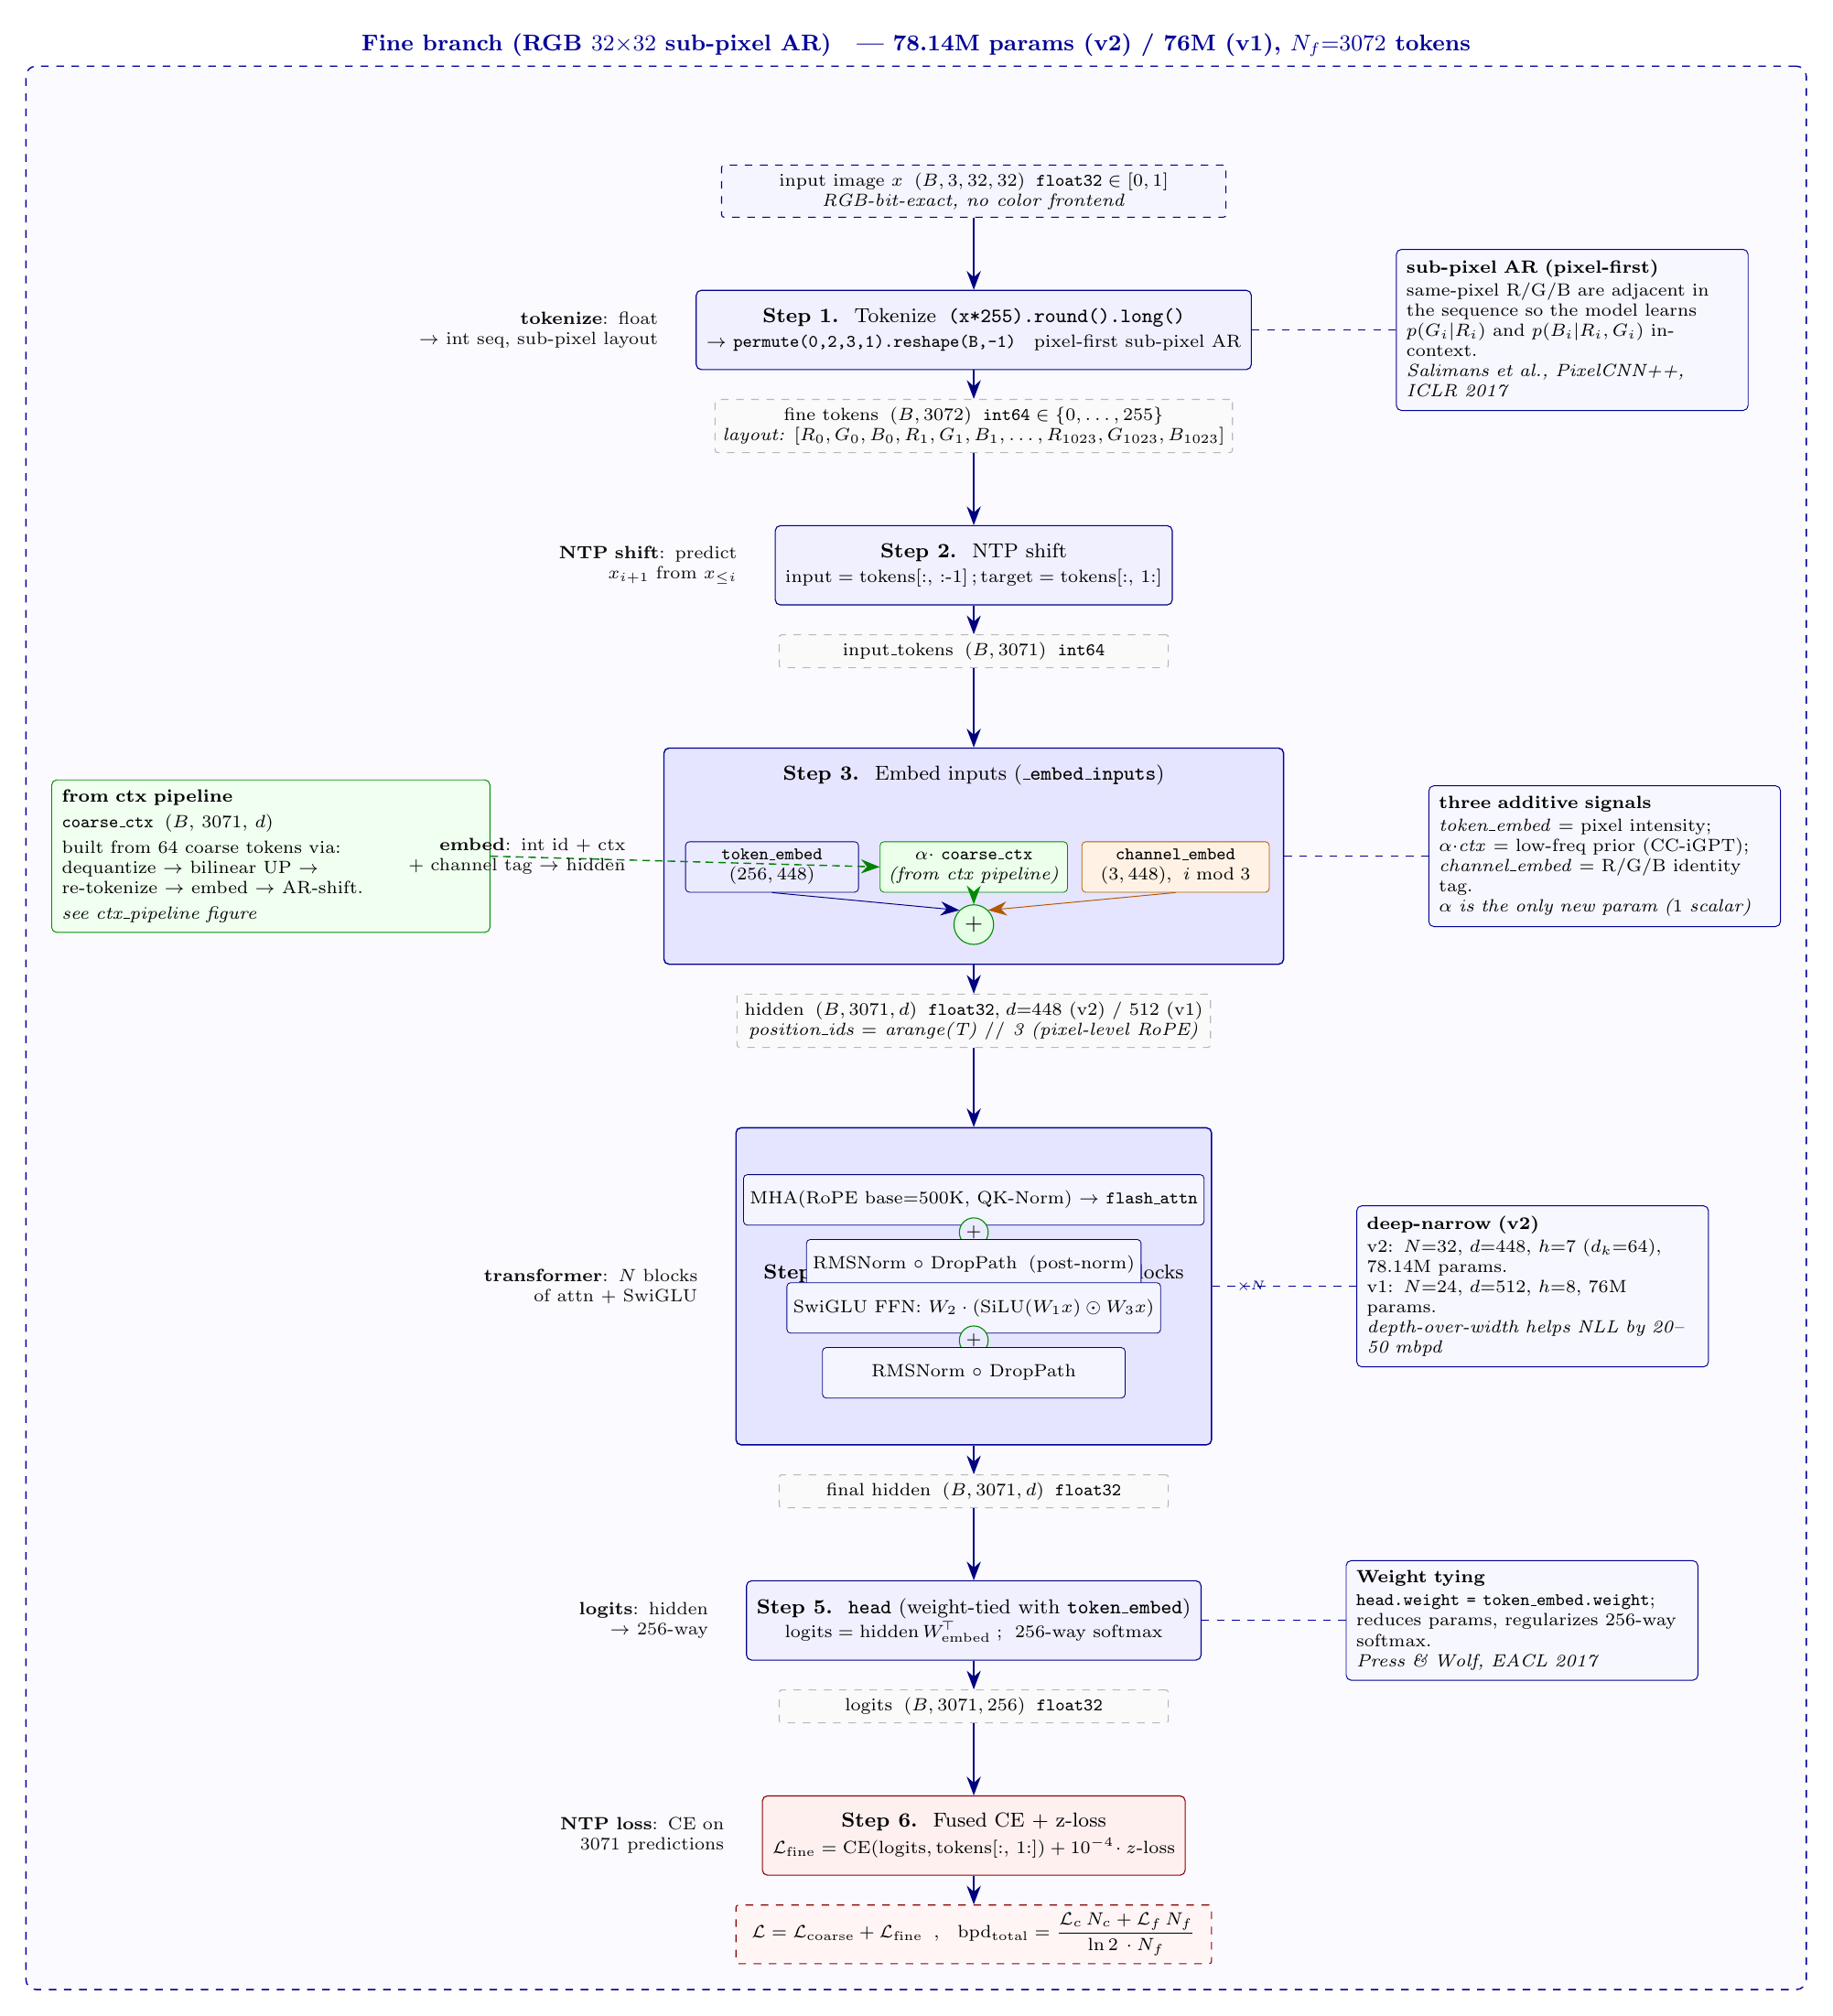
\begin{tikzpicture}[
    font=\footnotesize,
    >={Stealth[length=2.6mm]},
    node distance=10mm and 14mm,
    stepbox/.style ={draw, rounded corners=2pt, align=center,
                     minimum height=11mm, minimum width=54mm,
                     inner sep=4pt, fill=blue!6, draw=blue!55!black,
                     line width=0.4pt},
    blockbox/.style={draw, rounded corners=2pt, align=center,
                     minimum height=14mm, minimum width=54mm,
                     inner sep=4pt, fill=blue!10, draw=blue!60!black,
                     line width=0.5pt},
    sublayer/.style={draw, rounded corners=1.5pt, align=center,
                     minimum height=7mm, minimum width=36mm,
                     inner sep=2.5pt, fill=blue!4, draw=blue!50!black,
                     font=\scriptsize, line width=0.3pt},
    tensor/.style  ={draw, dashed, rounded corners=1pt, align=center,
                     fill=gray!4, draw=gray!55, font=\scriptsize,
                     inner sep=3pt, minimum width=54mm},
    lossbox/.style ={draw, rounded corners=2pt, align=center,
                     minimum height=11mm, minimum width=54mm,
                     inner sep=4pt, fill=red!6, draw=red!55!black,
                     line width=0.4pt},
    callout/.style ={draw=blue!60!black, rounded corners=2pt,
                     fill=blue!3, align=left, font=\scriptsize,
                     inner sep=4pt, line width=0.35pt},
    inject/.style  ={draw, circle, inner sep=0.5pt, fill=green!10,
                     draw=green!55!black, minimum size=5.5mm, font=\small},
    flow/.style    ={->, line width=0.55pt, blue!50!black},
    sidearrow/.style={->, line width=0.5pt, green!50!black, densely dashed},
]

% =========================================================
% TOP: invisible top spacer to host the fnbox label safely
% =========================================================
\node[minimum width=70mm, minimum height=8mm, inner sep=0pt]
     (topspacer) {};

% =========================================================
% TOP: input image
% =========================================================
\node[tensor, fill=blue!4, draw=blue!55!black, minimum width=70mm,
      below=2mm of topspacer]
     (xin) {input image $x$\;\;$(B,3,32,32)$\;\;\texttt{float32}\;$\in[0,1]$\\
            \textit{RGB-bit-exact, no color frontend}};

% =========================================================
% Step 1 -- tokenize (sub-pixel AR, pixel-first)
% =========================================================
\node[stepbox, below=10mm of xin] (s1)
     {\textbf{Step 1.} \;Tokenize\;\;\texttt{(x*255).round().long()}\\
      \scriptsize $\to$ \texttt{permute(0,2,3,1).reshape(B,-1)}\;\;
      pixel-first sub-pixel AR};
\node[tensor, below=4mm of s1] (t1)
     {fine tokens\;\;$(B,3072)$\;\;\texttt{int64}\;$\in\{0,\dots,255\}$\\
      \textit{layout: $[R_0,G_0,B_0,R_1,G_1,B_1,\dots,R_{1023},G_{1023},B_{1023}]$}};

% =========================================================
% Step 2 -- NTP shift
% =========================================================
\node[stepbox, below=10mm of t1] (s2)
     {\textbf{Step 2.} \;NTP shift\\
      \scriptsize input\;$=$\;tokens[:, :-1]\,;\,target\;$=$\;tokens[:, 1:]};
\node[tensor, below=4mm of s2] (t2)
     {input\_tokens\;\;$(B,3071)$\;\;\texttt{int64}};

% =========================================================
% Step 3 -- THREE additive injections (key composite step)
% =========================================================
\node[blockbox, below=11mm of t2, minimum height=30mm,
      minimum width=86mm] (s3) {};

% Title pinned to the top of the box so the three sublayers below don't overlap it
\node[anchor=north, font=\footnotesize, align=center, inner sep=1pt]
     at ($(s3.north)+(0,-2mm)$)
     {\textbf{Step 3.} \;Embed inputs (\texttt{\_embed\_inputs})};

% Three sub-injections inside Step 3 (shifted down into the lower half of the box)
\node[sublayer, fill=blue!8, minimum width=24mm]
     at ($(s3.center)+(-28mm,-1.5mm)$)
     (e_tok) {\texttt{token\_embed}\\$(256, 448)$};
\node[sublayer, fill=green!8, draw=green!55!black, minimum width=26mm]
     at ($(s3.center)+(0mm,-1.5mm)$)
     (e_ctx) {$\alpha\cdot$ \texttt{coarse\_ctx}\\\textit{(from ctx pipeline)}};
\node[sublayer, fill=orange!10, draw=orange!70!black, minimum width=26mm]
     at ($(s3.center)+(28mm,-1.5mm)$)
     (e_ch) {\texttt{channel\_embed}\\$(3, 448)$,\;\;$i\bmod 3$};

\node[inject] at ($(s3.center)+(0mm,-9.5mm)$) (plus) {$+$};
\draw[->, line width=0.35pt, blue!50!black] (e_tok.south) -- (plus.north west);
\draw[->, line width=0.35pt, green!55!black] (e_ctx.south) -- (plus.north);
\draw[->, line width=0.35pt, orange!70!black] (e_ch.south) -- (plus.north east);

\node[tensor, below=4mm of s3] (t3)
     {hidden\;\;$(B,3071,d)$\;\;\texttt{float32},\;$d{=}448$ (v2) / $512$ (v1)\\
      \textit{position\_ids $=$ arange(T) $//$ 3 (pixel-level RoPE)}};

% =========================================================
% Step 4 -- N stacked GPT blocks (with internal expansion)
% =========================================================
\node[blockbox, below=11mm of t3, minimum height=44mm,
      minimum width=66mm] (s4)
     {\textbf{Step 4.} \;Fine iGPT\;\;$N$ stacked GPT blocks\\
      \scriptsize $N{=}32$ (v2) / $24$ (v1),\;\;OLMo-2 post-norm};

% Internal block structure (one block expanded)
\node[sublayer, fill=blue!4] at ($(s4.center)+(0mm,12mm)$)
     (lay_attn) {MHA(RoPE base$=$500K, QK-Norm) $\to$ \texttt{flash\_attn}};
\node[inject, fill=blue!8, minimum size=4mm] at ($(s4.center)+(0mm,7.5mm)$)
     (add1) {\scriptsize$+$};
\node[sublayer, fill=blue!4, minimum width=42mm]
     at ($(s4.center)+(0mm,3mm)$)
     (lay_norm1) {RMSNorm $\circ$ DropPath\;\;(post-norm)};
\node[sublayer, fill=blue!4] at ($(s4.center)+(0mm,-3mm)$)
     (lay_ff)
     {SwiGLU FFN: $W_2 \cdot (\mathrm{SiLU}(W_1 x) \odot W_3 x)$};
\node[inject, fill=blue!8, minimum size=4mm] at ($(s4.center)+(0mm,-7.5mm)$)
     (add2) {\scriptsize$+$};
\node[sublayer, fill=blue!4, minimum width=42mm]
     at ($(s4.center)+(0mm,-12mm)$)
     (lay_norm2) {RMSNorm $\circ$ DropPath};

\node[font=\tiny, blue!55!black, anchor=west]
     at ($(s4.east)+(1.5mm,0)$)
     {\;$\times N$};

\node[tensor, below=4mm of s4] (t4)
     {final hidden\;\;$(B,3071,d)$\;\;\texttt{float32}};

% =========================================================
% Step 5 -- output head (weight-tied)
% =========================================================
\node[stepbox, below=10mm of t4] (s5)
     {\textbf{Step 5.} \;\texttt{head} (weight-tied with \texttt{token\_embed})\\
      \scriptsize $\text{logits} = \text{hidden}\,W^{\!\top}_{\text{embed}}$\;;\;
      256-way softmax};
\node[tensor, below=4mm of s5] (t5)
     {logits\;\;$(B,3071,256)$\;\;\texttt{float32}};

% =========================================================
% Step 6 -- loss
% =========================================================
\node[lossbox, below=10mm of t5] (s6)
     {\textbf{Step 6.} \;Fused CE + z-loss\\[1pt]
      \scriptsize $\mathcal{L}_{\text{fine}} = \mathrm{CE}(\text{logits},
      \text{tokens[:, 1:]}) + 10^{-4}\!\cdot z\text{-loss}$};
\node[tensor, below=4mm of s6, fill=red!4, draw=red!55!black,
      minimum width=66mm]
     (out) {$\mathcal{L} = \mathcal{L}_{\text{coarse}} + \mathcal{L}_{\text{fine}}$\;\;,\;\;
            $\mathrm{bpd_{total}} = \dfrac{\mathcal{L}_{c}\,N_c + \mathcal{L}_{f}\,N_f}
                                          {\ln 2\,\cdot N_f}$};

% =========================================================
% Side input: ctx pipeline feeds into Step 3
% =========================================================
\node[callout, left=24mm of s3, anchor=east, text width=58mm,
      fill=green!6, draw=green!55!black]
     (ctxIn) {\textbf{from ctx pipeline}\\[2pt]
              \texttt{coarse\_ctx}\;\;$(B,\,3071,\,d)$\\[2pt]
              built from $64$ coarse tokens via:\\
              dequantize $\to$ bilinear UP $\to$\\
              re-tokenize $\to$ embed $\to$ AR-shift.\\[2pt]
              \textit{see ctx\_pipeline figure}};
\draw[sidearrow] (ctxIn.east) -- (e_ctx.west);

% =========================================================
% Right callouts
% =========================================================
\node[callout, right=20mm of s1, anchor=west, text width=46mm]
     (caTok) {\textbf{sub-pixel AR (pixel-first)}\\[1pt]
              same-pixel R/G/B are adjacent in the sequence so the model
              learns $p(G_i|R_i)$ and $p(B_i|R_i,G_i)$ in-context.\\
              \textit{Salimans et al., PixelCNN++, ICLR 2017}};
\draw[blue!60!black, dashed, line width=0.35pt]
     (s1.east) -- (caTok.west);

\node[callout, right=20mm of s3, anchor=west, text width=46mm]
     (caInj) {\textbf{three additive signals}\\[1pt]
              \emph{token\_embed} = pixel intensity;\\
              \emph{$\alpha\cdot$ctx} = low-freq prior (CC-iGPT);\\
              \emph{channel\_embed} = R/G/B identity tag.\\
              \textit{$\alpha$ is the only new param ($1$ scalar)}};
\draw[blue!60!black, dashed, line width=0.35pt]
     (s3.east) -- (caInj.west);

\node[callout, right=20mm of s4, anchor=west, text width=46mm]
     (caBlk) {\textbf{deep-narrow (v2)}\\[1pt]
              v2: $N{=}32$, $d{=}448$, $h{=}7$ ($d_k{=}64$), 78.14M params.\\
              v1: $N{=}24$, $d{=}512$, $h{=}8$, 76M params.\\
              \textit{depth-over-width helps NLL by 20--50 mbpd}};
\draw[blue!60!black, dashed, line width=0.35pt]
     (s4.east) -- (caBlk.west);

\node[callout, right=20mm of s5, anchor=west, text width=46mm]
     (caHead) {\textbf{Weight tying}\\[1pt]
              \texttt{head.weight = token\_embed.weight}; reduces params,
              regularizes 256-way softmax.\\
              \textit{Press \& Wolf, EACL 2017}};
\draw[blue!60!black, dashed, line width=0.35pt]
     (s5.east) -- (caHead.west);

% =========================================================
% Left annotations
% =========================================================
\node[font=\scriptsize, gray!10!black, anchor=east, align=right,
      text width=46mm] (n1) at ($(s1.west)+(-4mm,0)$)
     {\textbf{tokenize}: float\\$\to$ int seq, sub-pixel layout};
\node[font=\scriptsize, gray!10!black, anchor=east, align=right,
      text width=46mm] (n2) at ($(s2.west)+(-4mm,0)$)
     {\textbf{NTP shift}: predict\\$x_{i+1}$ from $x_{\le i}$};
\node[font=\scriptsize, gray!10!black, anchor=east, align=right,
      text width=46mm] (n3) at ($(s3.west)+(-4mm,0)$)
     {\textbf{embed}: int id $+$ ctx\\$+$ channel tag $\to$ hidden};
\node[font=\scriptsize, gray!10!black, anchor=east, align=right,
      text width=46mm] (n4) at ($(s4.west)+(-4mm,0)$)
     {\textbf{transformer}: $N$ blocks\\of attn $+$ SwiGLU};
\node[font=\scriptsize, gray!10!black, anchor=east, align=right,
      text width=46mm] (n5) at ($(s5.west)+(-4mm,0)$)
     {\textbf{logits}: hidden\\$\to$ 256-way};
\node[font=\scriptsize, gray!10!black, anchor=east, align=right,
      text width=46mm] (n6) at ($(s6.west)+(-4mm,0)$)
     {\textbf{NTP loss}: CE on\\$3071$ predictions};

% =========================================================
% Main flow arrows
% =========================================================
\draw[flow] (xin) -- (s1);
\draw[flow] (s1) -- (t1);
\draw[flow] (t1) -- (s2);
\draw[flow] (s2) -- (t2);
\draw[flow] (t2) -- (s3);
\draw[flow] (s3) -- (t3);
\draw[flow] (t3) -- (s4);
\draw[flow] (s4) -- (t4);
\draw[flow] (t4) -- (s5);
\draw[flow] (s5) -- (t5);
\draw[flow] (t5) -- (s6);
\draw[flow] (s6) -- (out);

% =========================================================
% Background frame
% =========================================================
\begin{pgfonlayer}{background}
  \node[draw=blue!60!black, dashed, rounded corners=4pt,
        fill=blue!2, line width=0.5pt, inner sep=10pt,
        fit=(topspacer)(s1)(s6)(t1)(out)(caTok)(caInj)(caBlk)(caHead)(ctxIn)(n1)(n6),
        label={[blue!60!black, font=\small\bfseries]above:%
              \textbf{Fine branch (RGB $32{\times}32$ sub-pixel AR)} \;
              --- 78.14M params (v2) / 76M (v1), $N_f{=}3072$ tokens}]
        (fbox) {};
\end{pgfonlayer}

\end{tikzpicture}
\end{document}

%
% 配套 ctx_pipeline.tex / coarse_pipeline.tex，把 fine iGPT 分支 forward 全路径
% 在「张量 shape + dtype + 三路 additive 注入 + GPT block 内部」三个层面具象化。
\documentclass[tikz,border=10pt]{standalone}
\usepackage{tikz}
\usepackage{amsmath,amssymb}
\usepackage{xcolor}
\usetikzlibrary{positioning,arrows.meta,calc,fit,backgrounds,shapes.geometric,
                decorations.pathreplacing,patterns}

\begin{document}
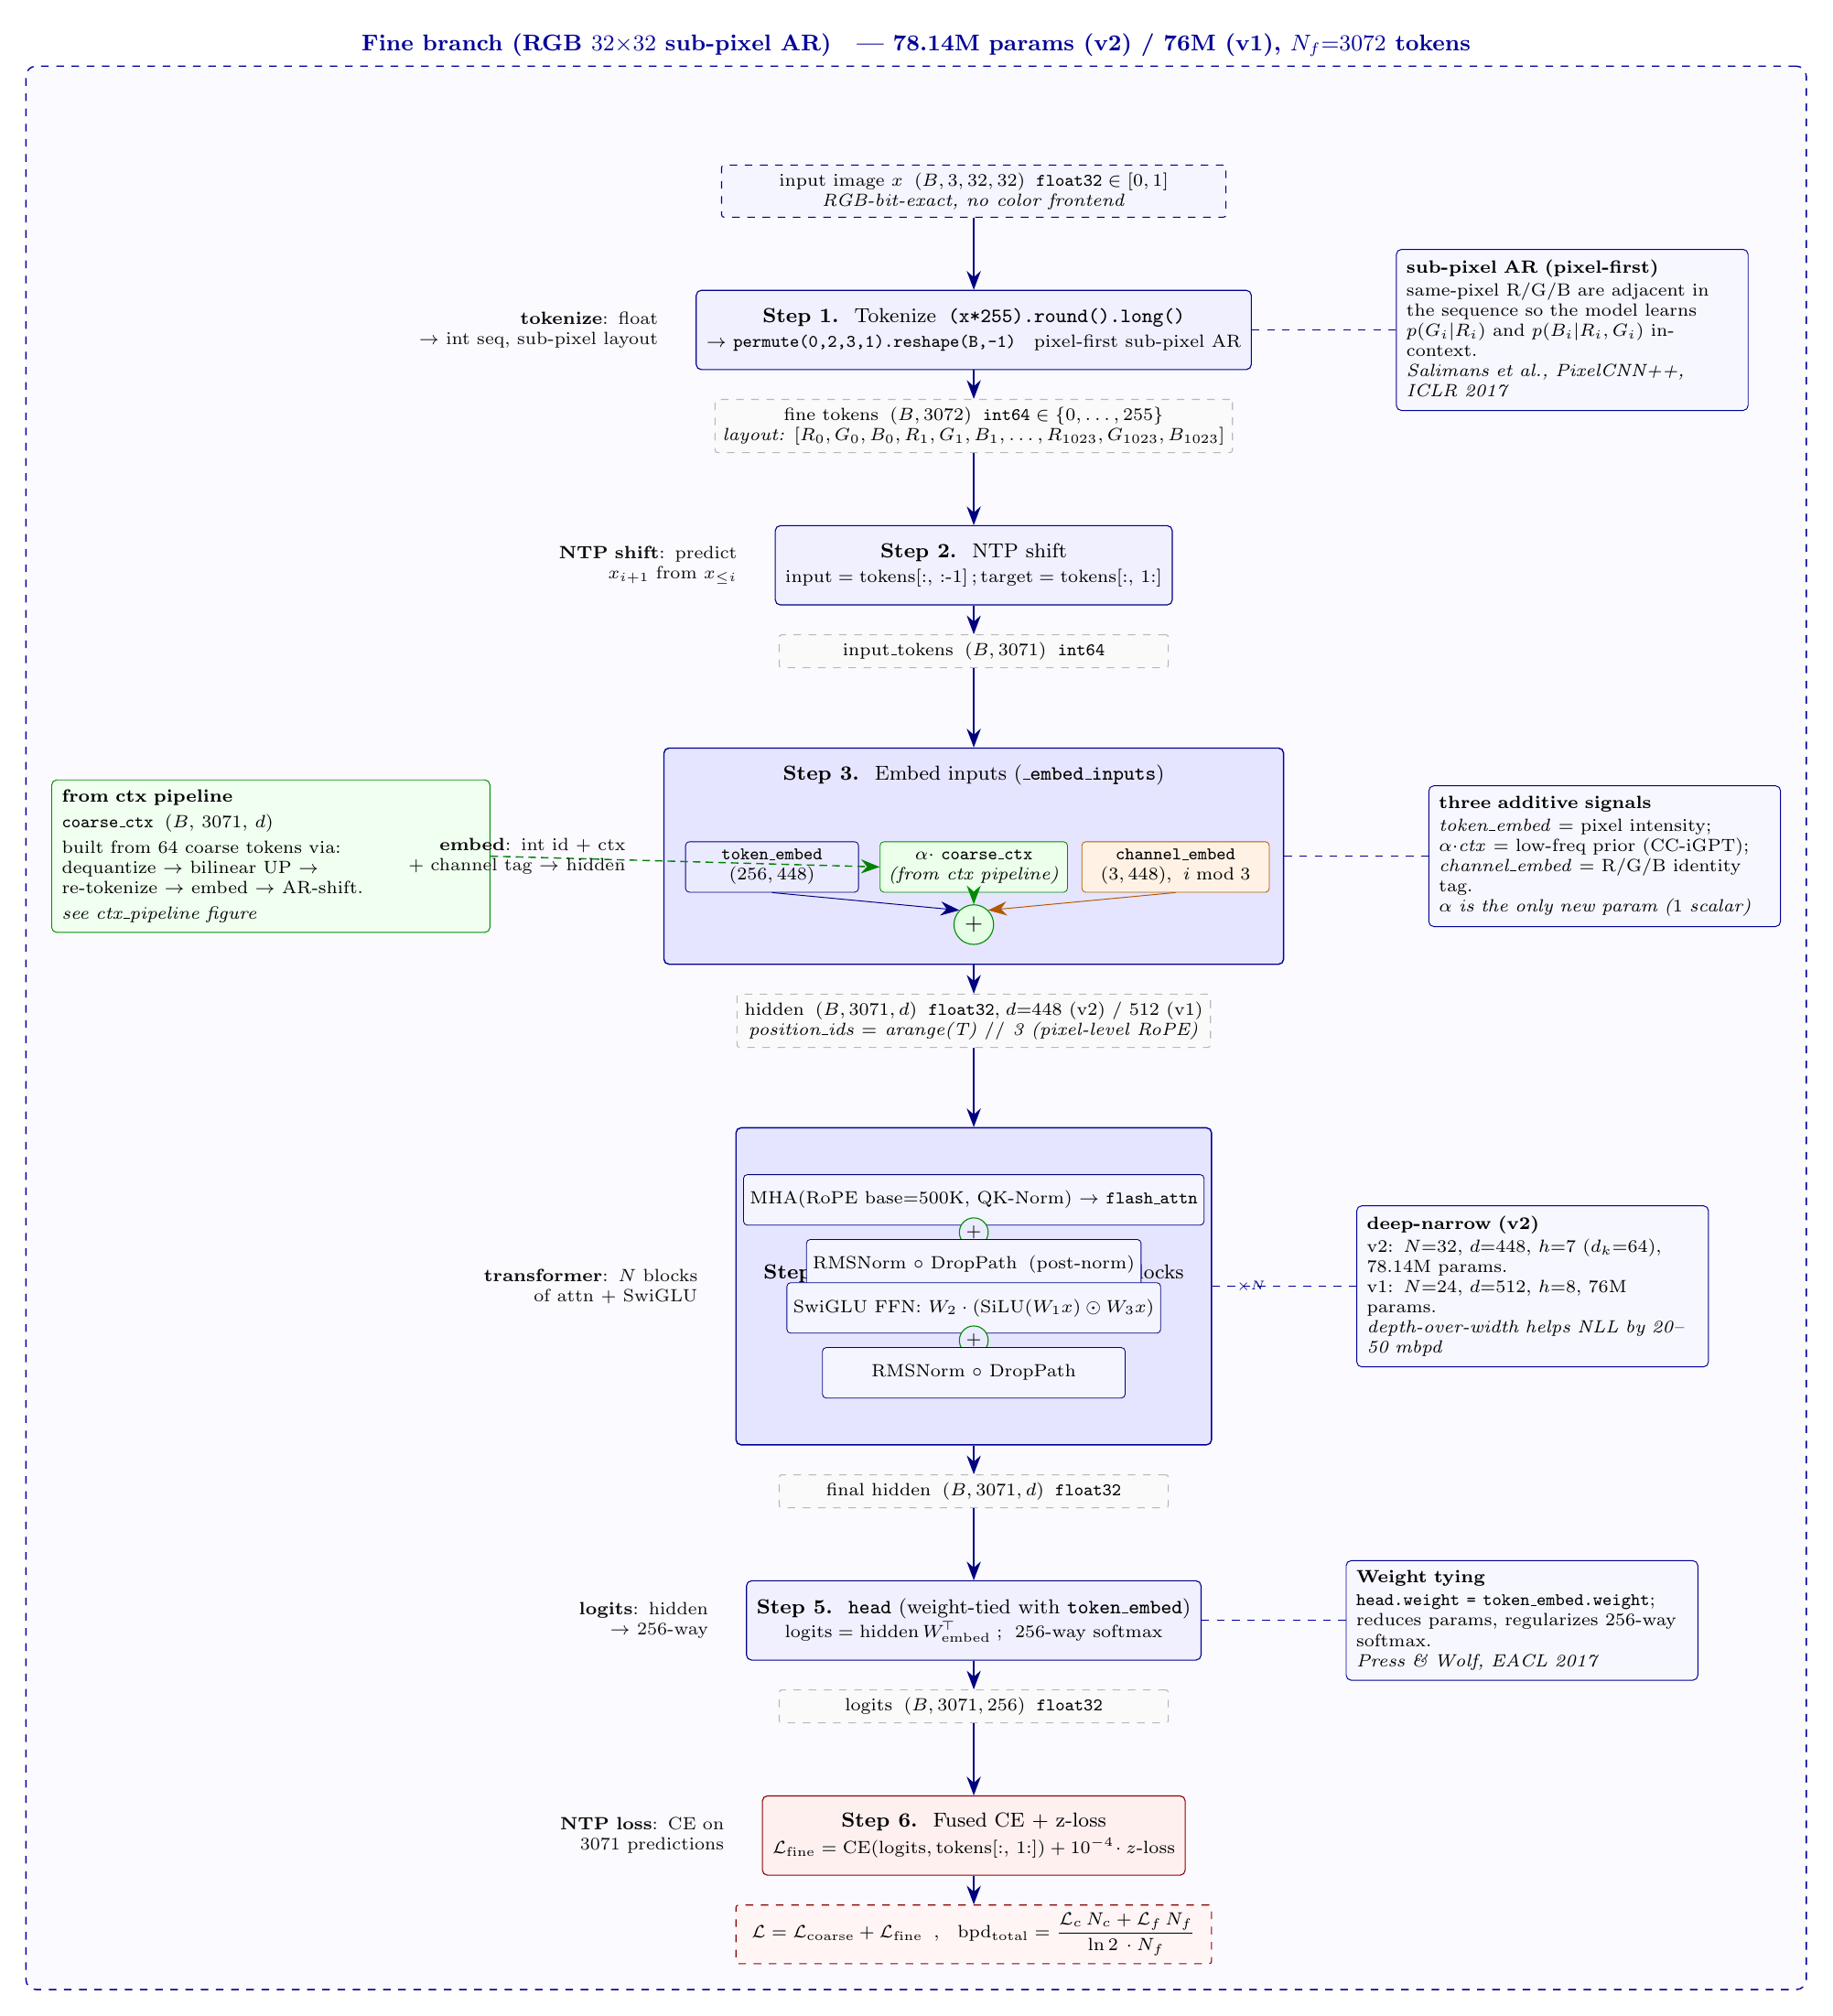
\begin{tikzpicture}[
    font=\footnotesize,
    >={Stealth[length=2.6mm]},
    node distance=10mm and 14mm,
    stepbox/.style ={draw, rounded corners=2pt, align=center,
                     minimum height=11mm, minimum width=54mm,
                     inner sep=4pt, fill=blue!6, draw=blue!55!black,
                     line width=0.4pt},
    blockbox/.style={draw, rounded corners=2pt, align=center,
                     minimum height=14mm, minimum width=54mm,
                     inner sep=4pt, fill=blue!10, draw=blue!60!black,
                     line width=0.5pt},
    sublayer/.style={draw, rounded corners=1.5pt, align=center,
                     minimum height=7mm, minimum width=36mm,
                     inner sep=2.5pt, fill=blue!4, draw=blue!50!black,
                     font=\scriptsize, line width=0.3pt},
    tensor/.style  ={draw, dashed, rounded corners=1pt, align=center,
                     fill=gray!4, draw=gray!55, font=\scriptsize,
                     inner sep=3pt, minimum width=54mm},
    lossbox/.style ={draw, rounded corners=2pt, align=center,
                     minimum height=11mm, minimum width=54mm,
                     inner sep=4pt, fill=red!6, draw=red!55!black,
                     line width=0.4pt},
    callout/.style ={draw=blue!60!black, rounded corners=2pt,
                     fill=blue!3, align=left, font=\scriptsize,
                     inner sep=4pt, line width=0.35pt},
    inject/.style  ={draw, circle, inner sep=0.5pt, fill=green!10,
                     draw=green!55!black, minimum size=5.5mm, font=\small},
    flow/.style    ={->, line width=0.55pt, blue!50!black},
    sidearrow/.style={->, line width=0.5pt, green!50!black, densely dashed},
]

% =========================================================
% TOP: invisible top spacer to host the fnbox label safely
% =========================================================
\node[minimum width=70mm, minimum height=8mm, inner sep=0pt]
     (topspacer) {};

% =========================================================
% TOP: input image
% =========================================================
\node[tensor, fill=blue!4, draw=blue!55!black, minimum width=70mm,
      below=2mm of topspacer]
     (xin) {input image $x$\;\;$(B,3,32,32)$\;\;\texttt{float32}\;$\in[0,1]$\\
            \textit{RGB-bit-exact, no color frontend}};

% =========================================================
% Step 1 -- tokenize (sub-pixel AR, pixel-first)
% =========================================================
\node[stepbox, below=10mm of xin] (s1)
     {\textbf{Step 1.} \;Tokenize\;\;\texttt{(x*255).round().long()}\\
      \scriptsize $\to$ \texttt{permute(0,2,3,1).reshape(B,-1)}\;\;
      pixel-first sub-pixel AR};
\node[tensor, below=4mm of s1] (t1)
     {fine tokens\;\;$(B,3072)$\;\;\texttt{int64}\;$\in\{0,\dots,255\}$\\
      \textit{layout: $[R_0,G_0,B_0,R_1,G_1,B_1,\dots,R_{1023},G_{1023},B_{1023}]$}};

% =========================================================
% Step 2 -- NTP shift
% =========================================================
\node[stepbox, below=10mm of t1] (s2)
     {\textbf{Step 2.} \;NTP shift\\
      \scriptsize input\;$=$\;tokens[:, :-1]\,;\,target\;$=$\;tokens[:, 1:]};
\node[tensor, below=4mm of s2] (t2)
     {input\_tokens\;\;$(B,3071)$\;\;\texttt{int64}};

% =========================================================
% Step 3 -- THREE additive injections (key composite step)
% =========================================================
\node[blockbox, below=11mm of t2, minimum height=30mm,
      minimum width=86mm] (s3) {};

% Title pinned to the top of the box so the three sublayers below don't overlap it
\node[anchor=north, font=\footnotesize, align=center, inner sep=1pt]
     at ($(s3.north)+(0,-2mm)$)
     {\textbf{Step 3.} \;Embed inputs (\texttt{\_embed\_inputs})};

% Three sub-injections inside Step 3 (shifted down into the lower half of the box)
\node[sublayer, fill=blue!8, minimum width=24mm]
     at ($(s3.center)+(-28mm,-1.5mm)$)
     (e_tok) {\texttt{token\_embed}\\$(256, 448)$};
\node[sublayer, fill=green!8, draw=green!55!black, minimum width=26mm]
     at ($(s3.center)+(0mm,-1.5mm)$)
     (e_ctx) {$\alpha\cdot$ \texttt{coarse\_ctx}\\\textit{(from ctx pipeline)}};
\node[sublayer, fill=orange!10, draw=orange!70!black, minimum width=26mm]
     at ($(s3.center)+(28mm,-1.5mm)$)
     (e_ch) {\texttt{channel\_embed}\\$(3, 448)$,\;\;$i\bmod 3$};

\node[inject] at ($(s3.center)+(0mm,-9.5mm)$) (plus) {$+$};
\draw[->, line width=0.35pt, blue!50!black] (e_tok.south) -- (plus.north west);
\draw[->, line width=0.35pt, green!55!black] (e_ctx.south) -- (plus.north);
\draw[->, line width=0.35pt, orange!70!black] (e_ch.south) -- (plus.north east);

\node[tensor, below=4mm of s3] (t3)
     {hidden\;\;$(B,3071,d)$\;\;\texttt{float32},\;$d{=}448$ (v2) / $512$ (v1)\\
      \textit{position\_ids $=$ arange(T) $//$ 3 (pixel-level RoPE)}};

% =========================================================
% Step 4 -- N stacked GPT blocks (with internal expansion)
% =========================================================
\node[blockbox, below=11mm of t3, minimum height=44mm,
      minimum width=66mm] (s4)
     {\textbf{Step 4.} \;Fine iGPT\;\;$N$ stacked GPT blocks\\
      \scriptsize $N{=}32$ (v2) / $24$ (v1),\;\;OLMo-2 post-norm};

% Internal block structure (one block expanded)
\node[sublayer, fill=blue!4] at ($(s4.center)+(0mm,12mm)$)
     (lay_attn) {MHA(RoPE base$=$500K, QK-Norm) $\to$ \texttt{flash\_attn}};
\node[inject, fill=blue!8, minimum size=4mm] at ($(s4.center)+(0mm,7.5mm)$)
     (add1) {\scriptsize$+$};
\node[sublayer, fill=blue!4, minimum width=42mm]
     at ($(s4.center)+(0mm,3mm)$)
     (lay_norm1) {RMSNorm $\circ$ DropPath\;\;(post-norm)};
\node[sublayer, fill=blue!4] at ($(s4.center)+(0mm,-3mm)$)
     (lay_ff)
     {SwiGLU FFN: $W_2 \cdot (\mathrm{SiLU}(W_1 x) \odot W_3 x)$};
\node[inject, fill=blue!8, minimum size=4mm] at ($(s4.center)+(0mm,-7.5mm)$)
     (add2) {\scriptsize$+$};
\node[sublayer, fill=blue!4, minimum width=42mm]
     at ($(s4.center)+(0mm,-12mm)$)
     (lay_norm2) {RMSNorm $\circ$ DropPath};

\node[font=\tiny, blue!55!black, anchor=west]
     at ($(s4.east)+(1.5mm,0)$)
     {\;$\times N$};

\node[tensor, below=4mm of s4] (t4)
     {final hidden\;\;$(B,3071,d)$\;\;\texttt{float32}};

% =========================================================
% Step 5 -- output head (weight-tied)
% =========================================================
\node[stepbox, below=10mm of t4] (s5)
     {\textbf{Step 5.} \;\texttt{head} (weight-tied with \texttt{token\_embed})\\
      \scriptsize $\text{logits} = \text{hidden}\,W^{\!\top}_{\text{embed}}$\;;\;
      256-way softmax};
\node[tensor, below=4mm of s5] (t5)
     {logits\;\;$(B,3071,256)$\;\;\texttt{float32}};

% =========================================================
% Step 6 -- loss
% =========================================================
\node[lossbox, below=10mm of t5] (s6)
     {\textbf{Step 6.} \;Fused CE + z-loss\\[1pt]
      \scriptsize $\mathcal{L}_{\text{fine}} = \mathrm{CE}(\text{logits},
      \text{tokens[:, 1:]}) + 10^{-4}\!\cdot z\text{-loss}$};
\node[tensor, below=4mm of s6, fill=red!4, draw=red!55!black,
      minimum width=66mm]
     (out) {$\mathcal{L} = \mathcal{L}_{\text{coarse}} + \mathcal{L}_{\text{fine}}$\;\;,\;\;
            $\mathrm{bpd_{total}} = \dfrac{\mathcal{L}_{c}\,N_c + \mathcal{L}_{f}\,N_f}
                                          {\ln 2\,\cdot N_f}$};

% =========================================================
% Side input: ctx pipeline feeds into Step 3
% =========================================================
\node[callout, left=24mm of s3, anchor=east, text width=58mm,
      fill=green!6, draw=green!55!black]
     (ctxIn) {\textbf{from ctx pipeline}\\[2pt]
              \texttt{coarse\_ctx}\;\;$(B,\,3071,\,d)$\\[2pt]
              built from $64$ coarse tokens via:\\
              dequantize $\to$ bilinear UP $\to$\\
              re-tokenize $\to$ embed $\to$ AR-shift.\\[2pt]
              \textit{see ctx\_pipeline figure}};
\draw[sidearrow] (ctxIn.east) -- (e_ctx.west);

% =========================================================
% Right callouts
% =========================================================
\node[callout, right=20mm of s1, anchor=west, text width=46mm]
     (caTok) {\textbf{sub-pixel AR (pixel-first)}\\[1pt]
              same-pixel R/G/B are adjacent in the sequence so the model
              learns $p(G_i|R_i)$ and $p(B_i|R_i,G_i)$ in-context.\\
              \textit{Salimans et al., PixelCNN++, ICLR 2017}};
\draw[blue!60!black, dashed, line width=0.35pt]
     (s1.east) -- (caTok.west);

\node[callout, right=20mm of s3, anchor=west, text width=46mm]
     (caInj) {\textbf{three additive signals}\\[1pt]
              \emph{token\_embed} = pixel intensity;\\
              \emph{$\alpha\cdot$ctx} = low-freq prior (CC-iGPT);\\
              \emph{channel\_embed} = R/G/B identity tag.\\
              \textit{$\alpha$ is the only new param ($1$ scalar)}};
\draw[blue!60!black, dashed, line width=0.35pt]
     (s3.east) -- (caInj.west);

\node[callout, right=20mm of s4, anchor=west, text width=46mm]
     (caBlk) {\textbf{deep-narrow (v2)}\\[1pt]
              v2: $N{=}32$, $d{=}448$, $h{=}7$ ($d_k{=}64$), 78.14M params.\\
              v1: $N{=}24$, $d{=}512$, $h{=}8$, 76M params.\\
              \textit{depth-over-width helps NLL by 20--50 mbpd}};
\draw[blue!60!black, dashed, line width=0.35pt]
     (s4.east) -- (caBlk.west);

\node[callout, right=20mm of s5, anchor=west, text width=46mm]
     (caHead) {\textbf{Weight tying}\\[1pt]
              \texttt{head.weight = token\_embed.weight}; reduces params,
              regularizes 256-way softmax.\\
              \textit{Press \& Wolf, EACL 2017}};
\draw[blue!60!black, dashed, line width=0.35pt]
     (s5.east) -- (caHead.west);

% =========================================================
% Left annotations
% =========================================================
\node[font=\scriptsize, gray!10!black, anchor=east, align=right,
      text width=46mm] (n1) at ($(s1.west)+(-4mm,0)$)
     {\textbf{tokenize}: float\\$\to$ int seq, sub-pixel layout};
\node[font=\scriptsize, gray!10!black, anchor=east, align=right,
      text width=46mm] (n2) at ($(s2.west)+(-4mm,0)$)
     {\textbf{NTP shift}: predict\\$x_{i+1}$ from $x_{\le i}$};
\node[font=\scriptsize, gray!10!black, anchor=east, align=right,
      text width=46mm] (n3) at ($(s3.west)+(-4mm,0)$)
     {\textbf{embed}: int id $+$ ctx\\$+$ channel tag $\to$ hidden};
\node[font=\scriptsize, gray!10!black, anchor=east, align=right,
      text width=46mm] (n4) at ($(s4.west)+(-4mm,0)$)
     {\textbf{transformer}: $N$ blocks\\of attn $+$ SwiGLU};
\node[font=\scriptsize, gray!10!black, anchor=east, align=right,
      text width=46mm] (n5) at ($(s5.west)+(-4mm,0)$)
     {\textbf{logits}: hidden\\$\to$ 256-way};
\node[font=\scriptsize, gray!10!black, anchor=east, align=right,
      text width=46mm] (n6) at ($(s6.west)+(-4mm,0)$)
     {\textbf{NTP loss}: CE on\\$3071$ predictions};

% =========================================================
% Main flow arrows
% =========================================================
\draw[flow] (xin) -- (s1);
\draw[flow] (s1) -- (t1);
\draw[flow] (t1) -- (s2);
\draw[flow] (s2) -- (t2);
\draw[flow] (t2) -- (s3);
\draw[flow] (s3) -- (t3);
\draw[flow] (t3) -- (s4);
\draw[flow] (s4) -- (t4);
\draw[flow] (t4) -- (s5);
\draw[flow] (s5) -- (t5);
\draw[flow] (t5) -- (s6);
\draw[flow] (s6) -- (out);

% =========================================================
% Background frame
% =========================================================
\begin{pgfonlayer}{background}
  \node[draw=blue!60!black, dashed, rounded corners=4pt,
        fill=blue!2, line width=0.5pt, inner sep=10pt,
        fit=(topspacer)(s1)(s6)(t1)(out)(caTok)(caInj)(caBlk)(caHead)(ctxIn)(n1)(n6),
        label={[blue!60!black, font=\small\bfseries]above:%
              \textbf{Fine branch (RGB $32{\times}32$ sub-pixel AR)} \;
              --- 78.14M params (v2) / 76M (v1), $N_f{=}3072$ tokens}]
        (fbox) {};
\end{pgfonlayer}

\end{tikzpicture}
\end{document}

%
% 配套 ctx_pipeline.tex / coarse_pipeline.tex，把 fine iGPT 分支 forward 全路径
% 在「张量 shape + dtype + 三路 additive 注入 + GPT block 内部」三个层面具象化。
\documentclass[tikz,border=10pt]{standalone}
\usepackage{tikz}
\usepackage{amsmath,amssymb}
\usepackage{xcolor}
\usetikzlibrary{positioning,arrows.meta,calc,fit,backgrounds,shapes.geometric,
                decorations.pathreplacing,patterns}

\begin{document}
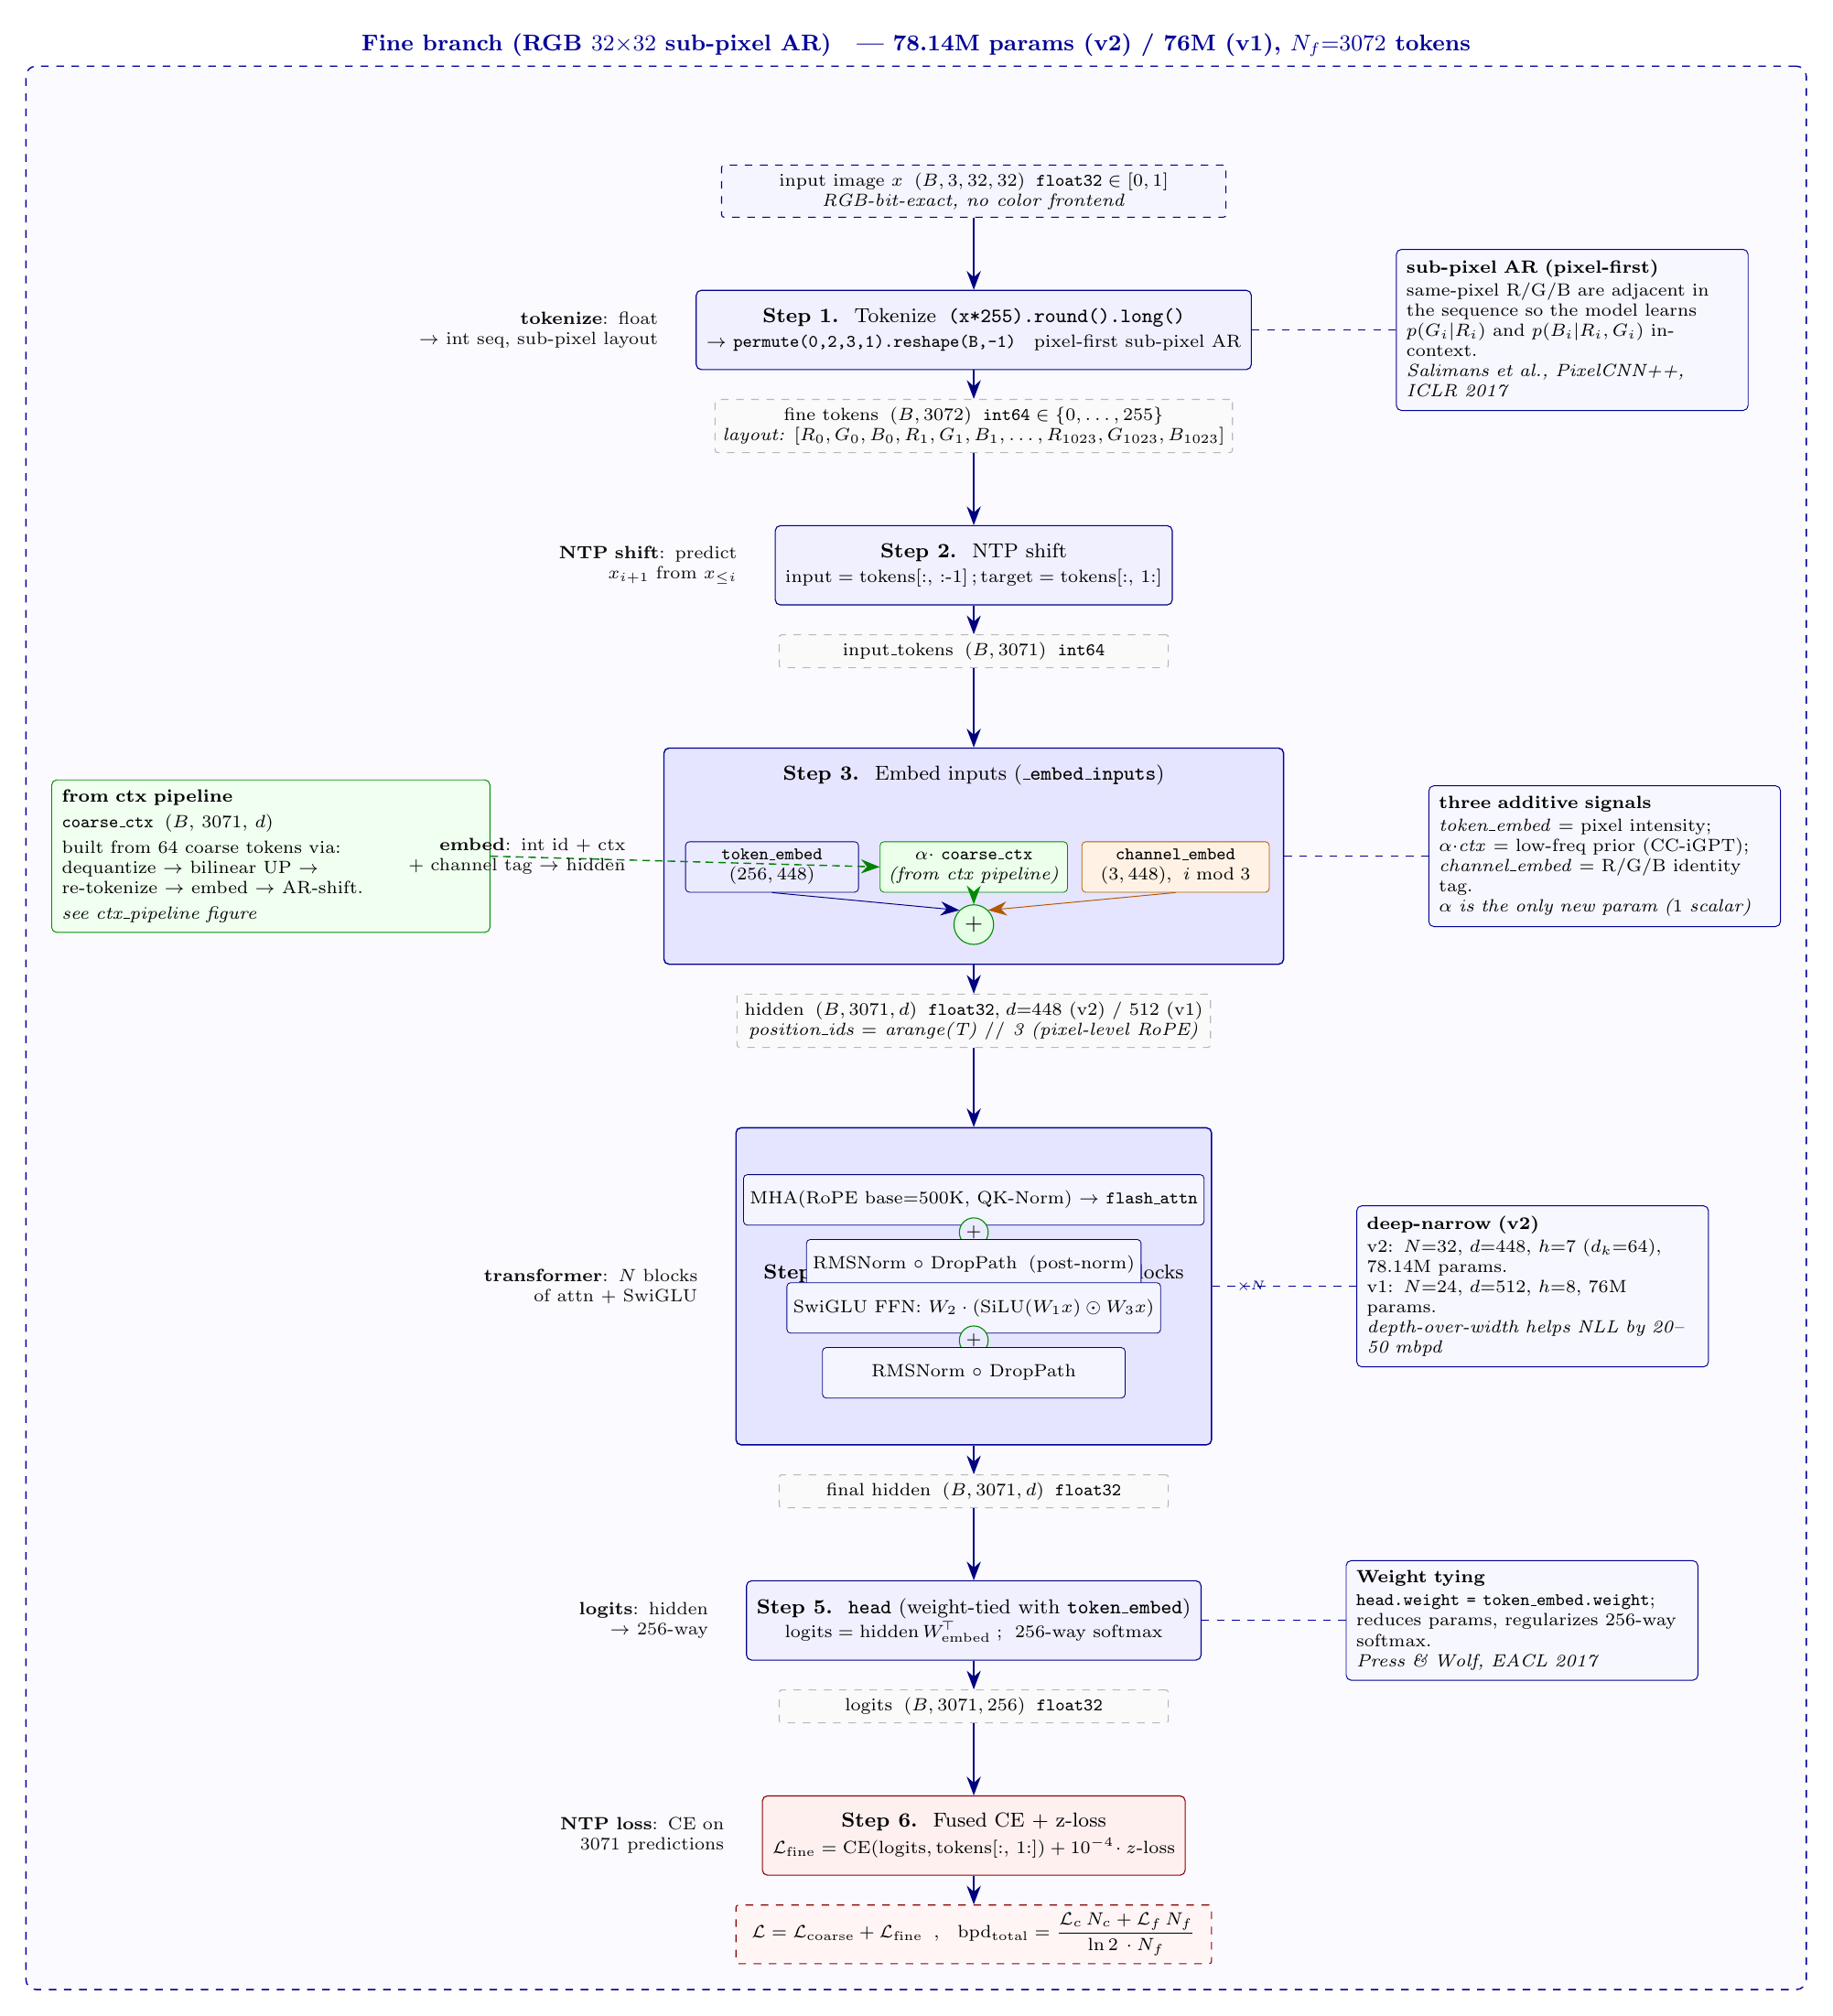
\begin{tikzpicture}[
    font=\footnotesize,
    >={Stealth[length=2.6mm]},
    node distance=10mm and 14mm,
    stepbox/.style ={draw, rounded corners=2pt, align=center,
                     minimum height=11mm, minimum width=54mm,
                     inner sep=4pt, fill=blue!6, draw=blue!55!black,
                     line width=0.4pt},
    blockbox/.style={draw, rounded corners=2pt, align=center,
                     minimum height=14mm, minimum width=54mm,
                     inner sep=4pt, fill=blue!10, draw=blue!60!black,
                     line width=0.5pt},
    sublayer/.style={draw, rounded corners=1.5pt, align=center,
                     minimum height=7mm, minimum width=36mm,
                     inner sep=2.5pt, fill=blue!4, draw=blue!50!black,
                     font=\scriptsize, line width=0.3pt},
    tensor/.style  ={draw, dashed, rounded corners=1pt, align=center,
                     fill=gray!4, draw=gray!55, font=\scriptsize,
                     inner sep=3pt, minimum width=54mm},
    lossbox/.style ={draw, rounded corners=2pt, align=center,
                     minimum height=11mm, minimum width=54mm,
                     inner sep=4pt, fill=red!6, draw=red!55!black,
                     line width=0.4pt},
    callout/.style ={draw=blue!60!black, rounded corners=2pt,
                     fill=blue!3, align=left, font=\scriptsize,
                     inner sep=4pt, line width=0.35pt},
    inject/.style  ={draw, circle, inner sep=0.5pt, fill=green!10,
                     draw=green!55!black, minimum size=5.5mm, font=\small},
    flow/.style    ={->, line width=0.55pt, blue!50!black},
    sidearrow/.style={->, line width=0.5pt, green!50!black, densely dashed},
]

% =========================================================
% TOP: invisible top spacer to host the fnbox label safely
% =========================================================
\node[minimum width=70mm, minimum height=8mm, inner sep=0pt]
     (topspacer) {};

% =========================================================
% TOP: input image
% =========================================================
\node[tensor, fill=blue!4, draw=blue!55!black, minimum width=70mm,
      below=2mm of topspacer]
     (xin) {input image $x$\;\;$(B,3,32,32)$\;\;\texttt{float32}\;$\in[0,1]$\\
            \textit{RGB-bit-exact, no color frontend}};

% =========================================================
% Step 1 -- tokenize (sub-pixel AR, pixel-first)
% =========================================================
\node[stepbox, below=10mm of xin] (s1)
     {\textbf{Step 1.} \;Tokenize\;\;\texttt{(x*255).round().long()}\\
      \scriptsize $\to$ \texttt{permute(0,2,3,1).reshape(B,-1)}\;\;
      pixel-first sub-pixel AR};
\node[tensor, below=4mm of s1] (t1)
     {fine tokens\;\;$(B,3072)$\;\;\texttt{int64}\;$\in\{0,\dots,255\}$\\
      \textit{layout: $[R_0,G_0,B_0,R_1,G_1,B_1,\dots,R_{1023},G_{1023},B_{1023}]$}};

% =========================================================
% Step 2 -- NTP shift
% =========================================================
\node[stepbox, below=10mm of t1] (s2)
     {\textbf{Step 2.} \;NTP shift\\
      \scriptsize input\;$=$\;tokens[:, :-1]\,;\,target\;$=$\;tokens[:, 1:]};
\node[tensor, below=4mm of s2] (t2)
     {input\_tokens\;\;$(B,3071)$\;\;\texttt{int64}};

% =========================================================
% Step 3 -- THREE additive injections (key composite step)
% =========================================================
\node[blockbox, below=11mm of t2, minimum height=30mm,
      minimum width=86mm] (s3) {};

% Title pinned to the top of the box so the three sublayers below don't overlap it
\node[anchor=north, font=\footnotesize, align=center, inner sep=1pt]
     at ($(s3.north)+(0,-2mm)$)
     {\textbf{Step 3.} \;Embed inputs (\texttt{\_embed\_inputs})};

% Three sub-injections inside Step 3 (shifted down into the lower half of the box)
\node[sublayer, fill=blue!8, minimum width=24mm]
     at ($(s3.center)+(-28mm,-1.5mm)$)
     (e_tok) {\texttt{token\_embed}\\$(256, 448)$};
\node[sublayer, fill=green!8, draw=green!55!black, minimum width=26mm]
     at ($(s3.center)+(0mm,-1.5mm)$)
     (e_ctx) {$\alpha\cdot$ \texttt{coarse\_ctx}\\\textit{(from ctx pipeline)}};
\node[sublayer, fill=orange!10, draw=orange!70!black, minimum width=26mm]
     at ($(s3.center)+(28mm,-1.5mm)$)
     (e_ch) {\texttt{channel\_embed}\\$(3, 448)$,\;\;$i\bmod 3$};

\node[inject] at ($(s3.center)+(0mm,-9.5mm)$) (plus) {$+$};
\draw[->, line width=0.35pt, blue!50!black] (e_tok.south) -- (plus.north west);
\draw[->, line width=0.35pt, green!55!black] (e_ctx.south) -- (plus.north);
\draw[->, line width=0.35pt, orange!70!black] (e_ch.south) -- (plus.north east);

\node[tensor, below=4mm of s3] (t3)
     {hidden\;\;$(B,3071,d)$\;\;\texttt{float32},\;$d{=}448$ (v2) / $512$ (v1)\\
      \textit{position\_ids $=$ arange(T) $//$ 3 (pixel-level RoPE)}};

% =========================================================
% Step 4 -- N stacked GPT blocks (with internal expansion)
% =========================================================
\node[blockbox, below=11mm of t3, minimum height=44mm,
      minimum width=66mm] (s4)
     {\textbf{Step 4.} \;Fine iGPT\;\;$N$ stacked GPT blocks\\
      \scriptsize $N{=}32$ (v2) / $24$ (v1),\;\;OLMo-2 post-norm};

% Internal block structure (one block expanded)
\node[sublayer, fill=blue!4] at ($(s4.center)+(0mm,12mm)$)
     (lay_attn) {MHA(RoPE base$=$500K, QK-Norm) $\to$ \texttt{flash\_attn}};
\node[inject, fill=blue!8, minimum size=4mm] at ($(s4.center)+(0mm,7.5mm)$)
     (add1) {\scriptsize$+$};
\node[sublayer, fill=blue!4, minimum width=42mm]
     at ($(s4.center)+(0mm,3mm)$)
     (lay_norm1) {RMSNorm $\circ$ DropPath\;\;(post-norm)};
\node[sublayer, fill=blue!4] at ($(s4.center)+(0mm,-3mm)$)
     (lay_ff)
     {SwiGLU FFN: $W_2 \cdot (\mathrm{SiLU}(W_1 x) \odot W_3 x)$};
\node[inject, fill=blue!8, minimum size=4mm] at ($(s4.center)+(0mm,-7.5mm)$)
     (add2) {\scriptsize$+$};
\node[sublayer, fill=blue!4, minimum width=42mm]
     at ($(s4.center)+(0mm,-12mm)$)
     (lay_norm2) {RMSNorm $\circ$ DropPath};

\node[font=\tiny, blue!55!black, anchor=west]
     at ($(s4.east)+(1.5mm,0)$)
     {\;$\times N$};

\node[tensor, below=4mm of s4] (t4)
     {final hidden\;\;$(B,3071,d)$\;\;\texttt{float32}};

% =========================================================
% Step 5 -- output head (weight-tied)
% =========================================================
\node[stepbox, below=10mm of t4] (s5)
     {\textbf{Step 5.} \;\texttt{head} (weight-tied with \texttt{token\_embed})\\
      \scriptsize $\text{logits} = \text{hidden}\,W^{\!\top}_{\text{embed}}$\;;\;
      256-way softmax};
\node[tensor, below=4mm of s5] (t5)
     {logits\;\;$(B,3071,256)$\;\;\texttt{float32}};

% =========================================================
% Step 6 -- loss
% =========================================================
\node[lossbox, below=10mm of t5] (s6)
     {\textbf{Step 6.} \;Fused CE + z-loss\\[1pt]
      \scriptsize $\mathcal{L}_{\text{fine}} = \mathrm{CE}(\text{logits},
      \text{tokens[:, 1:]}) + 10^{-4}\!\cdot z\text{-loss}$};
\node[tensor, below=4mm of s6, fill=red!4, draw=red!55!black,
      minimum width=66mm]
     (out) {$\mathcal{L} = \mathcal{L}_{\text{coarse}} + \mathcal{L}_{\text{fine}}$\;\;,\;\;
            $\mathrm{bpd_{total}} = \dfrac{\mathcal{L}_{c}\,N_c + \mathcal{L}_{f}\,N_f}
                                          {\ln 2\,\cdot N_f}$};

% =========================================================
% Side input: ctx pipeline feeds into Step 3
% =========================================================
\node[callout, left=24mm of s3, anchor=east, text width=58mm,
      fill=green!6, draw=green!55!black]
     (ctxIn) {\textbf{from ctx pipeline}\\[2pt]
              \texttt{coarse\_ctx}\;\;$(B,\,3071,\,d)$\\[2pt]
              built from $64$ coarse tokens via:\\
              dequantize $\to$ bilinear UP $\to$\\
              re-tokenize $\to$ embed $\to$ AR-shift.\\[2pt]
              \textit{see ctx\_pipeline figure}};
\draw[sidearrow] (ctxIn.east) -- (e_ctx.west);

% =========================================================
% Right callouts
% =========================================================
\node[callout, right=20mm of s1, anchor=west, text width=46mm]
     (caTok) {\textbf{sub-pixel AR (pixel-first)}\\[1pt]
              same-pixel R/G/B are adjacent in the sequence so the model
              learns $p(G_i|R_i)$ and $p(B_i|R_i,G_i)$ in-context.\\
              \textit{Salimans et al., PixelCNN++, ICLR 2017}};
\draw[blue!60!black, dashed, line width=0.35pt]
     (s1.east) -- (caTok.west);

\node[callout, right=20mm of s3, anchor=west, text width=46mm]
     (caInj) {\textbf{three additive signals}\\[1pt]
              \emph{token\_embed} = pixel intensity;\\
              \emph{$\alpha\cdot$ctx} = low-freq prior (CC-iGPT);\\
              \emph{channel\_embed} = R/G/B identity tag.\\
              \textit{$\alpha$ is the only new param ($1$ scalar)}};
\draw[blue!60!black, dashed, line width=0.35pt]
     (s3.east) -- (caInj.west);

\node[callout, right=20mm of s4, anchor=west, text width=46mm]
     (caBlk) {\textbf{deep-narrow (v2)}\\[1pt]
              v2: $N{=}32$, $d{=}448$, $h{=}7$ ($d_k{=}64$), 78.14M params.\\
              v1: $N{=}24$, $d{=}512$, $h{=}8$, 76M params.\\
              \textit{depth-over-width helps NLL by 20--50 mbpd}};
\draw[blue!60!black, dashed, line width=0.35pt]
     (s4.east) -- (caBlk.west);

\node[callout, right=20mm of s5, anchor=west, text width=46mm]
     (caHead) {\textbf{Weight tying}\\[1pt]
              \texttt{head.weight = token\_embed.weight}; reduces params,
              regularizes 256-way softmax.\\
              \textit{Press \& Wolf, EACL 2017}};
\draw[blue!60!black, dashed, line width=0.35pt]
     (s5.east) -- (caHead.west);

% =========================================================
% Left annotations
% =========================================================
\node[font=\scriptsize, gray!10!black, anchor=east, align=right,
      text width=46mm] (n1) at ($(s1.west)+(-4mm,0)$)
     {\textbf{tokenize}: float\\$\to$ int seq, sub-pixel layout};
\node[font=\scriptsize, gray!10!black, anchor=east, align=right,
      text width=46mm] (n2) at ($(s2.west)+(-4mm,0)$)
     {\textbf{NTP shift}: predict\\$x_{i+1}$ from $x_{\le i}$};
\node[font=\scriptsize, gray!10!black, anchor=east, align=right,
      text width=46mm] (n3) at ($(s3.west)+(-4mm,0)$)
     {\textbf{embed}: int id $+$ ctx\\$+$ channel tag $\to$ hidden};
\node[font=\scriptsize, gray!10!black, anchor=east, align=right,
      text width=46mm] (n4) at ($(s4.west)+(-4mm,0)$)
     {\textbf{transformer}: $N$ blocks\\of attn $+$ SwiGLU};
\node[font=\scriptsize, gray!10!black, anchor=east, align=right,
      text width=46mm] (n5) at ($(s5.west)+(-4mm,0)$)
     {\textbf{logits}: hidden\\$\to$ 256-way};
\node[font=\scriptsize, gray!10!black, anchor=east, align=right,
      text width=46mm] (n6) at ($(s6.west)+(-4mm,0)$)
     {\textbf{NTP loss}: CE on\\$3071$ predictions};

% =========================================================
% Main flow arrows
% =========================================================
\draw[flow] (xin) -- (s1);
\draw[flow] (s1) -- (t1);
\draw[flow] (t1) -- (s2);
\draw[flow] (s2) -- (t2);
\draw[flow] (t2) -- (s3);
\draw[flow] (s3) -- (t3);
\draw[flow] (t3) -- (s4);
\draw[flow] (s4) -- (t4);
\draw[flow] (t4) -- (s5);
\draw[flow] (s5) -- (t5);
\draw[flow] (t5) -- (s6);
\draw[flow] (s6) -- (out);

% =========================================================
% Background frame
% =========================================================
\begin{pgfonlayer}{background}
  \node[draw=blue!60!black, dashed, rounded corners=4pt,
        fill=blue!2, line width=0.5pt, inner sep=10pt,
        fit=(topspacer)(s1)(s6)(t1)(out)(caTok)(caInj)(caBlk)(caHead)(ctxIn)(n1)(n6),
        label={[blue!60!black, font=\small\bfseries]above:%
              \textbf{Fine branch (RGB $32{\times}32$ sub-pixel AR)} \;
              --- 78.14M params (v2) / 76M (v1), $N_f{=}3072$ tokens}]
        (fbox) {};
\end{pgfonlayer}

\end{tikzpicture}
\end{document}
